\mysection{Résultats}
\mysubsection{Scripts}
En dessous les résultats provenus des scripts crées dans la troisième partie du projet et après une bref discussion. 

\begin{itemize}
\item $\mathbf{gain\_calc-generator2bus}$\\
\begin{itemize}
	
\item $\mathbf{gain\_calc-generator2bus-test\_1-7am}$
\begin{table}[H]
	\captionsetup{justification=centering,margin=2cm}
	\caption{Matrice des Gain entre Puissance Réactive des générateurs et la tension des Bus ( Valeurs numériques )}
	\centering
	\begin{tabular}{ccc}
		1.7e-4&1.7e-4&1.7e-4\\
		1.7e-4&2.5e-4&2.7e-4\\
		1.7e-4&3.1e-4&2.4e-4\\
	\end{tabular}
\end{table}

\item $\mathbf{gain\_calc-generator2bus-test\_1-1pm}$
\begin{table}[H]
	\captionsetup{justification=centering,margin=2cm}
	\caption{Matrice des Gain entre Puissance Réactive des générateurs et la tension des Bus ( Valeurs numériques )}
	\centering
	\begin{tabular}{ccc}
		1.7e-4&1.7e-4&1.6e-4\\
		1.7e-4&2.4e-4&2.7e-4\\
		1.7e-4&3.0e-4&2.4e-4\\
	\end{tabular}
	
\end{table}

\item $\mathbf{gain\_calc-generator2bus-test\_2}$
\begin{table}[H]
	\captionsetup{justification=centering,margin=2cm}
	\caption{Matrice des Gain entre Puissance Réactive des générateurs et la tension des Bus ( Valeurs numériques )}
	\centering
	\begin{tabular}{ccc}
		
		1.8e-4&1.8e-4&1.7e-4\\
		
		1.8e-4&2.5e-4&2.8e-4\\
		
		1.8e-4&3.1e-4&2.5e-4\\
	\end{tabular}
\end{table}
\item $\mathbf{gain\_calc-load2bus}$\\
\\A cause de sa taille, la table des résultats \ref{tab:matrice_gain_load2bus} sont dans une autre page.
\\
\end{itemize}
\item $\mathbf{teste\_simul}$\\
\\ Testé sans régulateur on peut voir le gain négative du système \ref{fig:Puissance_Active_et_Reactive_de_la_Charge_C2_29_MT} et \ref{fig:Tension_des_Bus_N21_N23_et_N29}.\\
\begin{minipage}{.475\textwidth}
\begin{figure}[H]
	\begin{center}
		\captionsetup{justification=centering,margin=.5cm}	
		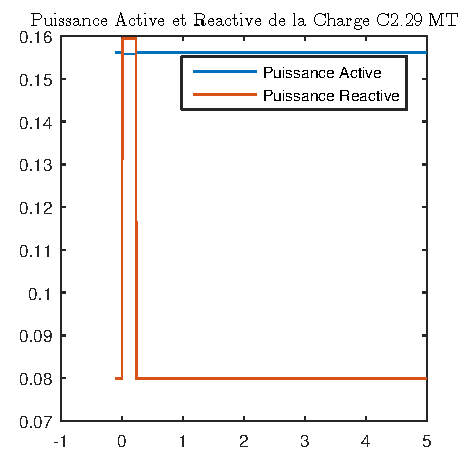
\includegraphics[width=\textwidth]{Resultats/Puissance_Active_et_Reactive_de_la_Charge_C2_29_MT.pdf}
		\caption{Puissance Active et Réactive \\de la Charge C2 29 MT}
		\label{fig:Puissance_Active_et_Reactive_de_la_Charge_C2_29_MT}
	\end{center}
\end{figure}
\end{minipage}
\begin{minipage}{.475\textwidth}
\begin{figure}[H]
	\begin{center}
		\captionsetup{justification=centering,margin=.5cm}	
		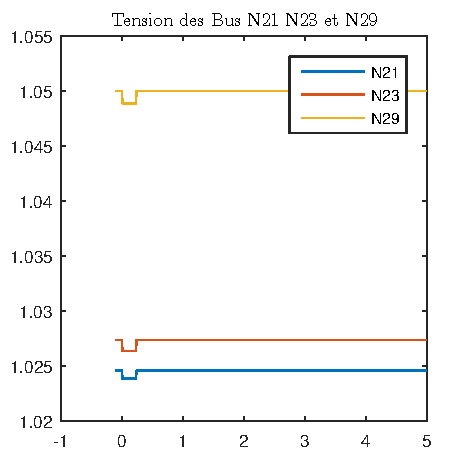
\includegraphics[width=\textwidth]{Resultats/Tension_des_Bus_N21_N23_et_N29.pdf}
		\caption{Tension des Bus N21 N23 et N29 en p.u.}
		\label{fig:Tension_des_Bus_N21_N23_et_N29}
	\end{center}
\end{figure}
\end{minipage}
\end{itemize}

\begin{sidewaysfigure}
	\begin{table}[H]\tiny
		\captionsetup{justification=centering,margin=2cm}
		\caption{Matrice des Gain entre Puissance Réactive des charges et la tension des Bus ( Valeurs numériques )}
		\label{tab:matrice_gain_load2bus}
		\centering
		\resizebox{\textwidth}{!}{\begin{tabular}{ccccccccccccccccc}
				%	1&2&3&4&5&6&7&8&9&10&11&12&13&14&15&16\\
				0e+0& -9.0e-5& -1.1e-4& -1.1e-4& -1.1e-4& -1.1e-4& -1.1e-4& -1.1e-4& -1.1e-4& -1.1e-4& -1.1e-4& -1.1e-4& -1.1e-4& -1.1e-4& -1.1e-4& -1.1e-4\\
				0e+0& -8.9e-5& -1.1e-4& -1.3e-4& -1.3e-4& -1.3e-4& -1.3e-4& -1.3e-4& -1.3e-4& -1.3e-4& -1.3e-4& -1.3e-4& -1.3e-4& -1.3e-4& -1.3e-4& -1.3e-4\\
				0e+0& -9.1e-5& -1.1e-4& -1.3e-4& -1.8e-4& -1.8e-4& -1.8e-4& -1.8e-4& -1.8e-4& -1.8e-4& -1.8e-4& -1.8e-4& -1.8e-4& -1.8e-4& -1.8e-4& -1.8e-4\\
				0e+0& -1.2e-4& -1.5e-4& -1.8e-4& -2.5e-4& -3.5e-4& -4.2e-4& -4.2e-4& -4.2e-4& -4.2e-4& -4.2e-4& -3.4e-4& -3.4e-4& -3.4e-4& -3.4e-4& -3.4e-4\\
				0e+0& -9.4e-5& -1.2e-4& -1.4e-4& -1.9e-4& -2.7e-4& -3.3e-4& -3.9e-4& -3.9e-4& -3.9e-4& -3.9e-4& -2.6e-4& -2.6e-4& -2.6e-4& -2.6e-4& -2.6e-4\\
				0e+0& -9.5e-5& -1.2e-4& -1.4e-4& -1.9e-4& -2.7e-4& -3.3e-4& -4.0e-4& -4.3e-4& -4.3e-4& -4.3e-4& -2.7e-4& -2.6e-4& -2.6e-4& -2.7e-4& -2.7e-4\\
				0e+0& -9.3e-5& -1.2e-4& -1.4e-4& -1.9e-4& -2.6e-4& -3.2e-4& -3.8e-4& -4.2e-4& -4.5e-4& -4.5e-4& -2.6e-4& -2.6e-4& -2.6e-4& -2.6e-4& -2.6e-4\\
				0e+0& 0e+0& 0e+0& 0e+0& 0e+0& 0e+0& 0e+0& 0e+0& 0e+0& 0e+0& 0e+0& 0e+0& 0e+0& 0e+0& 0e+0& 0e+0\\
				0e+0& 0e+0& 0e+0& 0e+0& 0e+0& 0e+0& 0e+0& 0e+0& 0e+0& 0e+0& 0e+0& 0e+0& 0e+0& 0e+0& 0e+0& 0e+0\\
				0e+0& -9.7e-5& -1.2e-4& -1.4e-4& -2.0e-4& -2.7e-4& -3.4e-4& -4.0e-4& -4.4e-4& -4.8e-4& -5.2e-4& -2.7e-4& -2.7e-4& -2.7e-4& -2.7e-4& -2.7e-4\\
				0e+0& -9.5e-5& -1.2e-4& -1.4e-4& -1.9e-4& -2.7e-4& -2.7e-4& -2.7e-4& -2.7e-4& -2.7e-4& -2.7e-4& -2.8e-4& -2.8e-4& -2.8e-4& -2.8e-4& -2.8e-4\\
				0e+0& -9.1e-5& -1.1e-4& -1.3e-4& -1.9e-4& -2.6e-4& -2.6e-4& -2.6e-4& -2.6e-4& -2.6e-4& -2.6e-4& -2.7e-4& -2.8e-4& -2.8e-4& -2.9e-4& -2.9e-4\\
				0e+0& -9.5e-5& -1.2e-4& -1.4e-4& -1.9e-4& -2.7e-4& -2.7e-4& -2.7e-4& -2.7e-4& -2.7e-4& -2.7e-4& -2.8e-4& -3.0e-4& -3.1e-4& -3.1e-4& -3.1e-4\\
				0e+0& -9.3e-5& -1.2e-4& -1.4e-4& -1.9e-4& -2.6e-4& -2.6e-4& -2.7e-4& -2.7e-4& -2.7e-4& -2.7e-4& -2.8e-4& -2.9e-4& -3.1e-4& -3.2e-4& -3.2e-4\\
				0e+0& 0e+0& 0e+0& 0e+0& 0e+0& 0e+0& 0e+0& 0e+0& 0e+0& 0e+0& 0e+0& 0e+0& 0e+0& 0e+0& 0e+0& 0e+0\\
				0e+0& -9.2e-5& -1.2e-4& -1.4e-4& -1.9e-4& -2.6e-4& -2.6e-4& -2.6e-4& -2.6e-4& -2.6e-4& -2.6e-4& -2.8e-4& -2.9e-4& -3.0e-4& -3.2e-4& -3.4e-4
				\\
		\end{tabular}}
	\end{table} 
	
\end{sidewaysfigure}
\vspace{1em}
On peut voir a partir de ces données que le réseau est caractérisée pour les équations démontrés en \cite{cosson:tel-01374469}, la tension du bus a un gain positif par rapport a puissance réactive du générateur, correspondant au qu'on espère pour la bonne réponse du régulateur.

\mysubsection{Simulations avec le régulateur}
Comme les réponses étaient les mêmes entre les modèles Powerfactory,\\ Powerfactory$ \leftrightarrows $MATLAB et Powerfactory$ \leftrightarrows $MATLAB$ \leftrightarrows $Simulink, on a choisi d'afficher les résultats du modèle Powerfactory$ \leftrightarrows $MATLAB, afin d'avoir encore la communication entre les deux logiciels.

 Ici se présentent les réponses des simulations et après une bref discussion sur les résultats.
